%%%%%%%%%%%%%%%%%%%%%%% file template.tex %%%%%%%%%%%%%%%%%%%%%%%%%
%
% This is a general template file for the LaTeX package SVJour3
% for Springer journals.          Springer Heidelberg 2010/09/16
%
% Copy it to a new file with a new name and use it as the basis
% for your article. Delete % signs as needed.
%
% This template includes a few options for different layouts and
% content for various journals. Please consult a previous issue of
% your journal as needed.
%
%%%%%%%%%%%%%%%%%%%%%%%%%%%%%%%%%%%%%%%%%%%%%%%%%%%%%%%%%%%%%%%%%%%
%
% First comes an example EPS file -- just ignore it and
% proceed on the \documentclass line
% your LaTeX will extract the file if required
\begin{filecontents*}{example.eps}
%!PS-Adobe-3.0 EPSF-3.0
%%BoundingBox: 19 19 221 221
%%CreationDate: Mon Sep 29 1997
%%Creator: programmed by hand (JK)
%%EndComments
gsave
newpath
  20 20 moveto
  20 220 lineto
  220 220 lineto
  220 20 lineto
closepath
2 setlinewidth
gsave
  .4 setgray fill
grestore
stroke
grestore
\end{filecontents*}
%
\RequirePackage{fix-cm}
%
%\documentclass{svjour3}                     % onecolumn (standard format)
%\documentclass[smallcondensed]{svjour3}     % onecolumn (ditto)
\documentclass[smallextended]{svjour3}       % onecolumn (second format)
%\documentclass[twocolumn]{svjour3}          % twocolumn
%
\smartqed  % flush right qed marks, e.g. at end of proof
%

\usepackage{graphicx}
\usepackage{amsmath}
\usepackage{algorithm}
\usepackage{algorithmic}
\renewcommand{\algorithmicrequire}{\textbf{Initialize:}}

\usepackage{verbatim} %TODO delete before submission
\usepackage[numbers]{natbib}%TODO delete before submission

%TODO Zitierweise ändern, sieht schrecklich aus
%
% \usepackage{mathptmx}      % use Times fonts if available on your TeX system
%
% insert here the call for the packages your document requires
%\usepackage{latexsym}
% etc.
%
% please place your own definitions here and don't use \def but
% \newcommand{}{}
%
% Insert the name of "your journal" with
% \journalname{myjournal}
%
\begin{document}

\title{Deep Deterministic Policy Gradients: Components and Extensions
%\thanks{Grants or other notes
%about the article that should go on the front page should be
%placed here. General acknowledgments should be placed at the end of the article.}
}
\subtitle{}

%\titlerunning{Short form of title}        % if too long for running head

\author{Yannik Frisch \and Tabea Wilke \and Maximilian Gehrke %etc.
}

%\authorrunning{Short form of author list} % if too long for running head

\institute{F. Author \at
              first address \\
              Tel.: +123-45-678910\\
              Fax: +123-45-678910\\
              \email{fauthor@example.com}           %  \\
%             \emph{Present address:} of F. Author  %  if needed
           \and
           S. Author \at
              second address
}

\date{Received: date / Accepted: date}
% The correct dates will be entered by the editor


\maketitle

\begin{abstract}
TODO
\keywords{DDPG \and DQN \and DPG}
% \PACS{PACS code1 \and PACS code2 \and more}
% \subclass{MSC code1 \and MSC code2 \and more}
\end{abstract}

\section{Introduction}
\label{sec:intro}
Deep Deterministic Policy Gradients (DDPG) arises from Deterministic Policy 
Gradients (DPG) and Deep Q-Learning (DQN). In the following we describe the 
underlying algorithms DPG and DQN and which aspects DDPG uses of both of them. 

\subsection{Deep Q-Learning}
\nocite{mnih2015human}
\nocite{mnih2013playing}
\label{sec:DQN}
The Deep Q-Network approach (DQN) [x] combines the approximation power of Neural Networks with traditional Q-learning.It enables solving the classic Reinforcement Learning problem of achieving the maximum expected reward over time, even for large state spaces (e.g. image frames). The algorithm is an off-policy, model-free approach and is able to find a close to optimal action-value function for many cases and from this a close to optimal deterministic policy by greedily selecting the action: $\pi(s)=\max_{a}Q^*(s,a)$. In terms of a formula the optimal action-value function is represented by
\[ 
Q^*(s_t,a_t)=\max_\pi E \left[
\sum_{t^{'}=t}^{T}\gamma^{t^{'}-t}r_{t^{'}}|s_t=s,
a_t=a, \pi \right] 
\]
%TODO E richtig darstellen
 where $\gamma\in[0,1)$ is called the \textit{Discount Factor}, controlling the agents preference for rewards closer or further away in time. Rewards later on in an episode will still have impact on the result but their influence decreases by the amount of time-steps required to reach them in the future.
By definition this optimal value function yields the \textit{Bellman Equation} [x] and can be reinterpreted as maximizing the current reward and the discounted action-value of the resulting state. In formula this gives:
\[
Q^*(s,a) = E_{s'\sim\epsilon}\left[
r + \gamma \max_{a'}Q^*(s',a')|s,a \right]
\]
%TODO E
For approximating the action-value function $Q(s,a|\theta)\approx Q^*(s,a)$ the approach uses a deep neural network, called the Q-Network.
The Q-Network can be trained by minimizing a sequence of loss functions $L_i(\theta_i)$, depending on it's weights:
\[
L_i(\theta_i)=E_{s,a\sim\rho(.),s'\sim\epsilon}
\left[\left(r+\gamma \max_{a'} Q(s', 
a'|\theta_{i-1})-Q(s,a|\theta_i)\right)^2\right] 
\]
%TODO E richtig machen
This loss function is similiar to the classical temporal-difference loss used in Q-Learning, but with approximated action-value functions instead of lookup-tables. Derivating this loss w.r.t. the approximation's weights gives:
\[
\nabla_{\theta_i}L_i(\theta_i)=E_{s,a\sim\rho(.),s'\sim\epsilon}
\left[\left(r+\gamma \max_{a'} Q(s', 
a'|\theta_{i-1})-Q(s,a|\theta_i)\right)\nabla_{\theta_i}Q(s,a|\theta_i)\right] 
\]
The expectation can be obtained by samling and this gradient can be used to optimize the loss function by using stochastic gradient descent.\\
Furthermore, a replay buffer is used which stores samples of the environment. This allows random mini-batch sampling, which decorrelates the samples and is proven to improve the performance by greater data efficiency [x]. The mini-batch sampling also enables the use of improved derivatives of vanilla stochastic gradient descent, e.g. \textit{RPROP} as in the \textit{neural fitted Q-Learning (NFQ)} [x] approach or \textit{ADAM update} [x].\\
%TODO Rewrite the target network stuff
There are different ways of estimating the expected Q-values. Either with a target network with the same structure as the network for the action-value function or the normal network. If a target network is used, the target weights need to be updated after some training steps.\\
A pseudocode for the DQN approach can be found in \ref{DQN-algo}.
The DQN approach was able to significantly outperform earlier learning methods despite incorporating almost no prior knowledge about the inputs [x], but is limited by the disabilty to cope with continous and high-dimensional action spaces due to the max operator in the action selection [x]. This limitations can be adressed by combining the approach with the Deterministic Policy Gradient, which is described in the following section.

\begin{algorithm}
	\caption{Deep Q-Learning (DQN)}\label{DQN-algo}
	\begin{algorithmic}
		\REQUIRE Replay buffer $\mathit{D}$ with high capacity
		\REQUIRE Neural network for action-value function $\mathit{Q}$
		with random weights $\theta$
		\REQUIRE Neural network for target action-value function$
		\mathit{\hat{Q}}$ with weights $\theta^-=\theta$
		\FOR{episode $1$ \TO $M$}
		\STATE reset environment to state $s_1$
		\FOR{$t=1$ \TO $T$}
		\IF{random $i \le \epsilon$}
		\STATE random action $a_t$
		\ELSE
		\STATE $a_t=\operatorname*{argmin}_a Q(s_t,a|\theta)$
		\ENDIF
		\STATE execute $a_t \rightarrow$ reward $r_t$ and next state 
		$s_{t+1}$
		\STATE save $(s_t, a_t, r_t,s_{t+1})$ in $D$
		\STATE sample minibatch $(s_i, a_i, r_i,s_{i+1})$ from $D$
		\STATE $q_i =
			\begin{cases}
			r_i & \textit{if episode terminates at step i+1}\\
			r_i+\gamma \max_{a'}\hat{Q}(s_{i+1}, a'|\theta^{-})& 
			else\\			
			\end{cases}$
		\STATE perform gradient descent on $\left(q_i-Q\left(s_i, 
		a_i|\theta\right)\right)^2_\theta$
		\STATE every $C$ steps update $\hat{Q}=Q$
		\ENDFOR
		\ENDFOR
	\end{algorithmic}
\end{algorithm}


\subsection{Deterministic Policy Gradient}
\label{sec:DPG}
\nocite{lillicrap2015continuous}
As [EDIT: QUELLE (ddpg paper)] stated correctly, most problems in reinforcement learning consist of a continuous action space which makes it very difficult to greedily choose the best action given a policy, due to the max operator. From a stochastic point of view, the policy is a probability distribution $a\sim\pi(a|s)$ over all actions. In order to calculate the gradient of a parameterized policy $\pi(a,s|\theta)$ over the total reward w.r.t. the weights, one needs to solve an integral over all actions and states, which becomes untractable for large state-action spaces.
From a deterministic view the policy is a discrete mapping from states to actions $a=\pi(s)$ and thus only one integration over the state space is sufficient.\\ 
%TODO Explain likelihood ratio gradients?
The \textit{policy gradient theorem} [EDIT: QUELLE (Sutton)] gives the update rule for a parameterized policy, optimizing the loss function: 
\[
\nabla_{\theta}J(\theta)=E_{s\sim\rho^\pi,a\sim\pi_\theta}
\left[\nabla_\theta log \pi_\theta(a|s)Q^\pi(s,a)\right] 
\]
From this, a deterministic approach is derived in [EDIT: by?] [EDIT: REFFERENCE (dpg paper)], which gives the update rule for a parameterized deterministic policy function $\pi(s|\theta)$. Rather than trying to maximize the action-value function $Q(s,a)$ globally by greedy improvements of the policy, the authors move the policy in the direction of the gradient of $Q(s,a)$:
\[
\nabla_{\theta^\pi}J\approx E_{s_t\sim\rho^\beta}\left[\nabla_{\theta^\pi}Q(s,a|\theta^Q)\right]
\]
%TODO s  ... Beta or Pi?
Applying the chain rule to this equation gives the \textit{deterministic policy gradient (DPG) theorem}:
\begin{align*}
\nabla_{\theta^\pi}J\approx E_{s_t\sim\rho^\beta}\left[\nabla_aQ(s,a|\theta^Q)|_{s=s_t,a=\pi(st)} \nabla_{\theta^\pi}\pi(s|\theta^\pi)|_{s=s_t}\right]
\end{align*}
where the expectation can again be obtained from sampling from an environment.
Only using deterministic action outputs will vanish the algorithms exploration, so one needs to make sure there still is exploration [EDIT: FORMULATION]. This is realized by using an off-policy approach which follows a stochastic behavior policy while learning about a deterministic target policy. The authors also introduce the notion of \textit{compatible function approximation}. Using these to extimate the gradient, an unbiased approximation is guaranteed.\\
The following section describes a typical structure of how to use deep neural networks for function approximation in reinforcement learning. Together with this section this led to the algorithm described in chapter \ref{sec:DDPG}.
%TODO Explain compatible FA?

%TODO Probleme mit DPG und nns beschreiben -> DDPG
\subsection{Actor-Critic Methods}
\label{sec:actor-critic}
A lot of recent success in reinforcement learning is based on \textit{Actor-Critic} methods [EDIT: REFFERENCE].
In contrast to value-function or policy-gradient methodes, they parameterize both, the value function $Q(s,a) \approx \hat{Q}(s,a|\theta^Q)$, also known as the \textit{Critic}, and the policy $\pi(s|a) \approx  \hat{\pi}(s|a,\theta^\pi)$. To get an intuition about these methods figure \ref{fig:actor-critic} illustrates the update-cycle:
\begin{figure}[H]
	\centering
	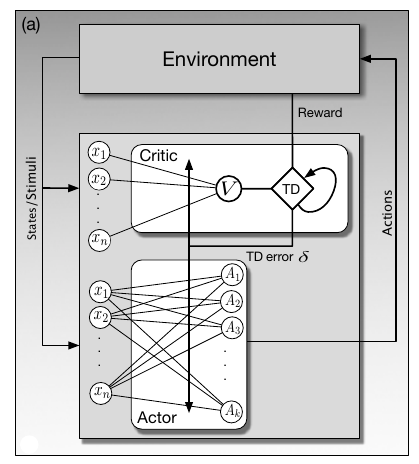
\includegraphics[width=0.4\linewidth]{actor-critic}
	\caption{Intuition about actor-critic methods (figure from 
	\cite{sutton2018reinforcement})}
	\label{fig:actor-critic}
\end{figure}
While the actor learns how to choose the right action and is responsible to update his policy, the critic has to learn and update the parameters of the state-value function. The actors' and the 
critics' parameters can be updated following the TD-error of the critic which is calculated from 
the observed reward and the current error of the estimated state values in every time-step. As Fig. 
\ref{fig:actor-critic} illustrates, the actor has no information about the 
current reward and the critic has no direct influence on the actions.  
%TODO direct influence richtig formuliert?
A pseudocode for an actor-critic method using TD-errors is shown in algorithm \ref{actor-critic-algo}.
\begin{algorithm}
	\caption{Episodic One-step Actor-Critic for Estimating $\pi(s|a,\theta^\pi) \approx \pi^*(s|a)$}\label{actor-critic-algo}
	\begin{algorithmic}
		\REQUIRE Differentiable policy parameterization $\pi(a|s,\theta^\pi)$
		\REQUIRE Differentiable action-value function parameterization $Q(s,a|\theta^Q)$
		\REQUIRE Random initial weights $\theta^\pi$ and $\theta^Q$
		\REQUIRE Step size parameters $\alpha^Q > 0$ and $\alpha^\pi >0$
		\REQUIRE Discount factor $\gamma$
		\FOR{episode $1$ \TO $M$}
		\STATE Get initial state s
		\STATE $i \leftarrow 1$
		\FOR{time-step 1 to T}
		\STATE{Draw action from actor: $a\sim\pi(s|a,\theta^\pi)$}
		\STATE{Do action a, observe reward r and successor state $s'$}
		\STATE{Calculate the TD-error:\\
		\qquad $\delta \leftarrow r + \gamma \max_a' Q(s',a'|\theta^Q) - Q(s,a|\theta^Q)$}
		%TODO Check if TD-error is correct for Q-Function
		\STATE{Update the weights:\\
		\qquad $\theta^Q \leftarrow \theta^Q + \alpha^Q\delta\nabla_{\theta^Q}Q(s,a|\theta^Q)$\\
		\qquad $\theta^\pi \leftarrow \theta^\pi + \alpha^\pi i \delta\nabla_{\theta^\pi}\log\pi(a|s,\theta^\pi)$}
		\STATE{Update:\\
		\qquad $i \leftarrow \gamma i$\\
		\qquad $s \leftarrow s'$}		
		\ENDFOR
		\ENDFOR
	\end{algorithmic}
\end{algorithm}

\section{Deep Deterministic Policy Gradient}
\label{sec:DDPG}
\nocite{lillicrap2015continuous}
The combination of above approaches led to the \textit{Deep Deterministic Policy Gradient (DDPG)} approach [x], which is a model-free and off-policy algorithm. It can be grouped into the class actor-critic methods and uses a deterministic target policy and deep Q-Learning. Both, the actor and the critic, are realized by deep neural networks. The pseudocode for DDPG can be found in \ref{DDPG-algo}.\\
It consists of a parameterized deterministic policy, the actor, $\pi(s|\theta^\pi)$ and a parameterized action-value function $Q(s,a|\theta^Q)$, the critic. The critic is updated using the \textit{Bellman Equation} with a TD-error similar in Q-Learning [EDIT: REFFERENCE] [EDIT: EQUATION?] and the actor is updated using the DPG theorem [EDIT: LINK? EQUATIONS WITH NUMBERS?].\\
The use of neural networks to parameterize the above functions means that the convergence guarantees do not hold anymore. Therefore the Actor-Critic DPG approach is combined with recent successes from DQN.\\
To ensure independently and identically distributed data, the authors use a replay buffer and sample random mini-batches from it. This again decorrelates the samples and allows the efficient use of hardware optimization, e.g. the ADAM update [EDIT: REFFERENCE].\\
To adress instability issues from applying deep neural network approximation to Q-Learning they also use \textit{target networks} which are copies of the actor $\pi'(s|\theta^{\pi'})$ and the critic $Q'(s,a|\theta^{Q'})$. These target-networks track the learned networks and are constrained to slow changes by using soft updates: $\theta' \leftarrow \tau\theta + (1-\tau)\theta'$ with $\tau << 1$. These consitent targets might slow down the learning process but greatly improve the stability of it.\\
Using low dimensional feature input might give very different scales for the single states. This can lead to problematic learning for the neural networks and is adresses by using \textit{batch normalization} which normalizes each dimension across the samples in a mini-batch.\\
To ensure exploration while using a deterministic policy, a noise process $\mathit{N}$ is added to the action output of the actor network. This noise process can be choosen to suit the environment. 
\begin{algorithm}
	\caption{Deep Deterministic Policy Gradient (DDPG)}\label{DDPG-algo}
	\begin{algorithmic}
		\REQUIRE Replay buffer $\mathit{D}$ with high capacity
		\REQUIRE Critic network $Q(s,a|\theta^Q)$ and actor network $\pi(s|\theta^\pi)$ with random weights $\theta^Q$ and $\theta^\pi$
		\REQUIRE Initialize target networks $Q'$ and $\pi'$ with weights $\theta^{Q'}\leftarrow\theta^Q$ and $\theta^{\pi'}\leftarrow\theta^\pi$
		\FOR{episode $1$ \TO $M$}
		\STATE Initialize random process $\mathit{N}$ for action exploration
		\STATE Reset environment to state $s_1$
		\FOR{$t=1$ \TO $T$}
		\STATE Select action $a_t = \pi(s_t|\theta^\pi) + \mathit{N}_t$ from local actor
		\STATE Execute action $a_t$ and observe reward $r_t$ and next state $s_{t+1}$
		\STATE Save $(s_t, a_t, r_t,s_{t+1})$ in replay buffer $D$
		\STATE Sample minibatch $(s_i, a_i, r_i,s_{i+1})$ from $D$
		\STATE Set TD-target from target networks:\\
		\qquad $y_i = r_i + \gamma Q'(s_{i+1}, \pi'(s_{i+1}|\theta^{\pi'})|\theta^{Q'})$
		\STATE Update the critic by minimizing the loss:\\
		\qquad $L=\frac{1}{N}\sum_i(y_i - Q(s_i,a_i|\theta^Q))^2$
		\STATE Update the actor using the sampled policy gradient:\\ 			\qquad $\nabla_{\theta^\pi}J \approx \frac{1}{N} \sum_i \nabla_a Q(s,a|\theta^Q)|_{s=s_i, a=\pi(s_i)}\nabla_{\theta^\pi}\pi(s|\theta^\pi)|_{s=s_i}$
		\STATE Update the target networks:\\
		\qquad $\theta^{Q'}\leftarrow \tau \theta^Q + (1-\tau)\theta^{Q'}$\\
		\qquad $\theta^{\pi'}\leftarrow \tau \theta^\pi + (1-\tau)\theta^{\pi'}$
		\ENDFOR
		\ENDFOR
	\end{algorithmic}
\end{algorithm}
The algorithm was evaluated on more than 20 simulated physical tasks using the same algorithm, network structures and hyperparameters, including classic control problems like the cart-pole environment. Using low-dimensional feature input, it was able to find policies performing really well on most of the tasks. Their performance is competitive with these found by a controller with full access to the environment. The algorithm is even able to find good policies using high dimensional pixel input. For simple tasks this is just as fast as using low dimensional state features.\\
The most challenging issues of the approach are his poor sample efficiency and some instabilites. We present some possible extensions to DDPG in the next chapter which might improve on these issues.
%TODO Write smth about performance, show some examples
\\
\\
\\
TODO:
\begin{itemize}
\item discretizing the action space often suffers from the course of dimensionality
\item naive extension of DPG with nns turns out to be unstable for challenging problems
\end{itemize}


\section{Improvements for DDPG}
\subsection{Using importance sampling to sample from the replay-buffer}
TODO
\subsection{Using Action Noise in Parameter Space}
Instead of adding noise to the action space to ensure exploration, one could add adaptive noise directly to the parameters of the neural network [EDIT: LINK TO AI BLOG?]. This would add some randomness into the parameters of the agent and therefore into the decission it makes, while still always fully depending on it's current observation about it's environment. This parameter noise makes an agent's exploration more consistent and results in a more effective exploration, increased performance and smoother behavior. 
\subsection{Evoluationary approaches?}
TODO
\subsection{Improvements of the deep neural network architectures}
TODO
\label{sec:1}

\section{Conclusion}
\label{sec:conclusion}
\begin{comment}

We propose several possible extensions and show their performance on a task.\\
Text with citations \cite{RefB} and \cite{RefJ}.
\subsection{Subsection title}
\label{sec:2}
as required. Don't forget to give each section
and subsection a unique label (see Sect.~\ref{sec:1}).
\paragraph{Paragraph headings} Use paragraph headings as needed.
\begin{equation}
a^2+b^2=c^2
\end{equation}

% For one-column wide figures use
\begin{figure}
% Use the relevant command to insert your figure file.
% For example, with the graphicx package use
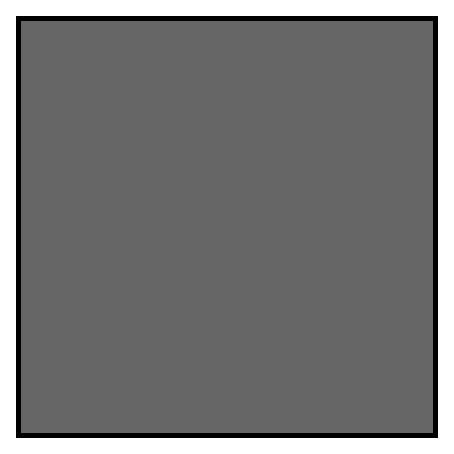
\includegraphics{example.eps}
% figure caption is below the figure
\caption{Please write your figure caption here}
\label{fig:1}       % Give a unique label
\end{figure}
%
% For two-column wide figures use
\begin{figure*}
% Use the relevant command to insert your figure file.
% For example, with the graphicx package use
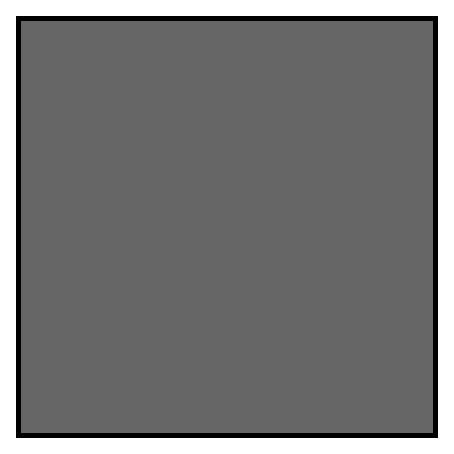
\includegraphics[width=0.75\textwidth]{example.eps}
% figure caption is below the figure
\caption{Please write your figure caption here}
\label{fig:2}       % Give a unique label
\end{figure*}


%
% For tables use
\begin{table}
% table caption is above the table
\caption{Please write your table caption here}
\label{tab:1}       % Give a unique label
% For LaTeX tables use
\begin{tabular}{lll}
\hline\noalign{\smallskip}
first & second & third  \\
\noalign{\smallskip}\hline\noalign{\smallskip}
number & number & number \\
number & number & number \\
\noalign{\smallskip}\hline
\end{tabular}
\end{table}


\end{comment}
%\begin{acknowledgements}
%If you'd like to thank anyone, place your comments here
%and remove the percent signs.
%\end{acknowledgements}

% BibTeX users please use one of
\bibliographystyle{spbasic}      % basic style, author-year citations
%\bibliographystyle{spmpsci}      % mathematics and physical sciences
%\bibliographystyle{spphys}       % APS-like style for physics
\bibliography{ddpg.bib}   % name your BibTeX data base

% Non-BibTeX users please use
\begin{comment}


\begin{thebibliography}{}
%
% and use \bibitem to create references. Consult the Instructions
% for authors for reference list style.
%
\bibitem{RefJ}
% Format for Journal Reference
Author, Article title, Journal, Volume, page numbers (year)
% Format for books
\bibitem{RefB}
Author, Book title, page numbers. Publisher, place (year)
% etc

\end{thebibliography}
\end{comment}
\end{document}
% end of file template.tex
